\documentclass{article}
\usepackage[margin=3cm]{geometry}
\usepackage{amssymb}

% Figures
\usepackage{graphicx}
\usepackage{color}

% Page formatting
\newsavebox{\notetitle}
\newsavebox{\noteauthor}
\newsavebox{\notenumber}
\newsavebox{\notedate}

\renewcommand{\title}[1]{\sbox{\notetitle}{\begin{minipage}{1.0\textwidth} \begin{center} \Large{\textbf{#1}} \end{center}\end{minipage} }}
%\renewcommand{\author}[1]{\renewcommand{\and}{\quad}\sbox{\noteauthor}{\large{#1}}}
\renewcommand{\author}[1]{\sbox{\noteauthor}{\begin{minipage}{1.0\textwidth} \begin{center} \large{#1} \end{center}\end{minipage}}}
\renewcommand{\date}[1]{\sbox{\notedate}{\large{#1}}}
\newcommand{\nb}[1]{\sbox{\notenumber}{\Large{\textbf{#1}}}}

\newcommand{\makemadtitle}{
  \hrule
  \vspace{.5em}
  \noindent
  \begin{center}
  \textbf{
  {\centering
\includegraphics[height=3cm,bb=0 0 371 145]{../logoCHISTERA2014.png}}\\
  %{\centering
\includegraphics[height=3cm]{../logoCHISTERA2014.eps}}\\
   {\centering\Large COACHES project, CHIST-ERA 2014 program}
  }
  \end{center}
  \vspace{.5em}
 
  \hrule
  \vspace{3em}
  \begin{center}
    %\begin{large}\textbf{ Note~\usebox{\notenumber}.}\end{large}\\[.5em]
    \begin{Large}\textbf{\usebox{\notetitle}}\end{Large}\\[2em]
    \begin{large}\usebox{\noteauthor}\\ [2em]
    \usebox{\notedate}\end{large}
  \end{center}
  \vspace{3em}
}

% Various macros and environments
\newtheorem{prop}{Proposition}
\newtheorem{proposition}[prop]{Proposition}
\newtheorem{defn}{Definition}
\newtheorem{definition}[defn]{Definition}
\newtheorem{cor}{Corollary}
\newtheorem{corollary}[cor]{Corollary}
\newtheorem{exmp}{Example}
\newtheorem{example}[exmp]{Example}
\newtheorem{lem}{Lemma}
\newtheorem{lemma}[lem]{Lemma}
\newtheorem{fact}{Fact}
\newtheorem{thm}{Theorem}
\newtheorem{theorem}[thm]{Theorem}
\newtheorem{prob}{Problem}
\newtheorem{problem}[prob]{Problem}
\newtheorem{rem}{Remark}
\newtheorem{remark}[rem]{Remark}
\newtheorem{conj}{Conjecture}
\newtheorem{conjecture}[conj]{Conjecture}
\newenvironment{pf}{{\bf Proof }}{\hfill$\Box$\par}
\newenvironment{proof}{{\bf Proof }}{\hfill$\Box$\par}
\newcommand{\spaceafterproof}{\vspace{1em}}

% NOTE ITSELF BELOW %%%%%%%%%%%%%%%%%%%%%%%%%%%%%%%%%%%%%%%%%%%%%

\title{D5.1-Sapienza\\ Definition of internal architecture and interface between software modules}

\author{Roberto Capobianco, Fabio Maria Carlucci, Giorgio Grisetti, Luca Iocchi, \\
Daniele Nardi, and Andrea Pennisi\\
\textit{Dept. of Computer, Control and Management Engineering\\
Sapienza University of Rome\\
via Ariosto, 25 00185 Rome, Italy}}


%\nb{of the kickoff meeting, $27^{th},28^{th}$ October }

\date{Version 1.0 - December 30, 2014}

\begin{document}


\includegraphics[height=3cm]{../logoSapienza.png}

\makemadtitle

\begin{abstract}
This document describes the software architecture of the entire project, showing the main software components, their connections and the interfaces between them.
\end{abstract}

\vspace*{2.0cm}

\fbox{
\begin{minipage}{1.0\textwidth}
\begin{center}
 $\copyright$, THE COACHES CONSORTIUM \\
The copyright in this document is the property of the COACHES Consortium. This document is supplied by the COACHES consortium on the express terms that it is to be treated as confidential. This document is not external distribution without the project manager's permission. 
\end{center}
\end{minipage}
}
\newpage

\begin{figure}
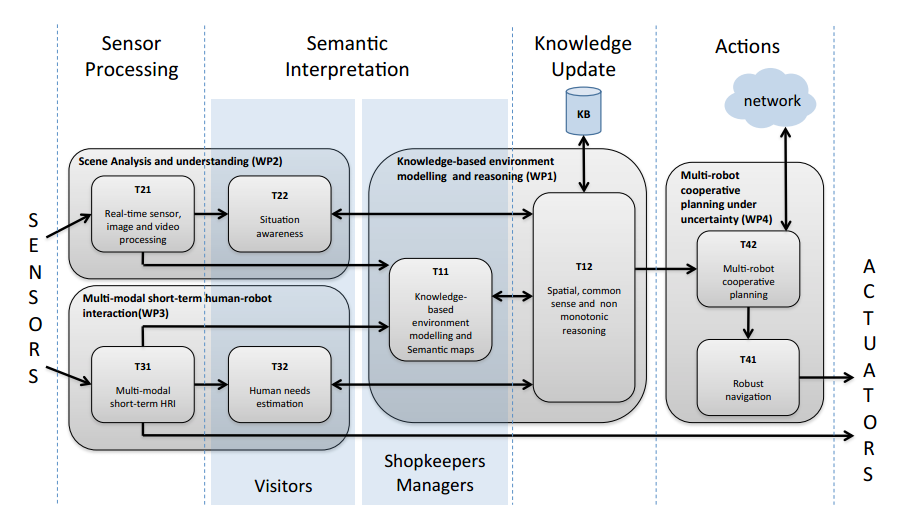
\includegraphics[width=0.95\textwidth]{COACHES_swarch.png}
\caption{COACHES software architecture}
\label{fig:swarch}
\end{figure}

\section{Introduction}

In this document the software architecture developed within the
context of the COACHES project is described.

Design solutions regarding the middleware chosen for implementing the entire system are discussed,
according to the modules shown in Fig. \ref{fig:swarch}).
Subsequent implementation of the software components during the project will follow  these  specifications,  thus  simplifying  their  integration  in  the demonstrators. 
A detailed description of the interface between the modules will be developed at a later stage, where more details on the single components will be provided.


An open architecture (hard/soft) and standard technologies available (such 
as ROS for integrating robotic modules and DDS for communication) will be used,
so that it will be 
easy to extend and/or adapt the capabilities of the system during the whole length of 
the  project  (especially  to  integrate  and  test  various  algorithms  and/or  sensors).  Such 
an open architecture will also simplify and optimize integration efficiency as well as re-use of assets in other projects or products. 

The reminder of this document is organized as follows.
First, the choice of the middleware is discussed, then the main software components and the
set-up of a 2D simulation environment and the collection of data sets for testing the developments are described.
Finally, the version management system that will be used to manage the development is illustrated.

\section{Middleware}

For the development of the software robotics components, the Robot Operating System (ROS)\footnote{www.ros.org}, which is the standard middleware for robotics applications, has been selected.
In particular, the last stable version ROS Indigo and the last LTS (Long Term Support) version of the Linux/Ubuntu Operating System will be used.

ROS provides the middleware to share information among the many modules implementing various functionalities on each robot. Moreover, an interface (ROS-through-TCP) will be realized in order to share information among the robots and between each robot and other components of the system.

\section{Main software components}

In this section, the main robotic software components that will be development for the control, the reasoning and the interaction functionalities of the robot are described.

\subsection{Robotic software components}

The main robotic software components that will be realized within the COACHES project are related to the following project tasks.
\begin{itemize}
\item T1.1 KB modeling
\item T1.2 KB reasoning
\item T2.1 Image Processing
\item T2.2 Situation Awareness
\item T3.1 Multimodal HRI
\item T3.2 Human needs estimation
\item T4.1 Robust navigation
\item T4.2 Multi-robot planning
\end{itemize}

Sapienza University is responsible for tasks T3.1 and T4.1. In Task T3.1 milti-modal human-robot interaction techniques will be implemented, including speech recognition and synthesis, people detection and tracking, people identification through the use of special markers (e.g., RFID or bar code reading).
In Task 4.1 techniques for safe navigation in a populated environment will be developed. Safety is of course of utmost importance in the project and thus we have defined different levels of security for the COACHES robots, as follows.

\begin{enumerate}
\item Hardware Emergency Stop button. Each robot is provided with two easy-to-access emergency stop button that will immediately cut current to motors in order to stop it.
\item Software Remote Emergency Stop. A wireless device (e.g., a wireless joystick) is configured to disable motor commands immediately, upon pushing a button, in the low-level software module.
\item Obstacle avoidance module. A software module using artificial potential fields for obstacle avoidance is always active.
\item Protection from hardware and software failures. All the low-level software modules are configured in order to immediately stop sending commands to the robot, if they detect any anomaly, such as a sensor not sending data or another software module not working properly. 
\end{enumerate}

\subsection{Interfaces between software components}

The main interfaces between the modules developed by Sapienza University and other modules in the system are the information collected through human-robot interaction (T3.1) to be used for the semantic map in Task T1.1. To this end, we have defined a specification of the semantic map, that will be used withing the reasoning system.

The semantic map of the environment is formed by two components: a metric map and a set of semantic annotations related to the metric map. The semantic annotations are expressed as predicates in a Prolog-like language. 
%An example of such a map is provided below.


\section{2D Simulation Environment}

The simulation environment is based on 2D Stage simulator, which is integrated in the ROS infrastructure. The choice of a 2D simulator (instead of a 3D one) is motivated by: 1) the need of modeling and testing high-level behaviors of the robot that does not involve 3D perception, 2) the possibility of using the simulator for multiple robots and other moving elements representing people in the environment, 3) the possibility of using the simulator on standard laptop, thus not requiring advanced graphical cards for running 3D simulations.

\begin{figure}
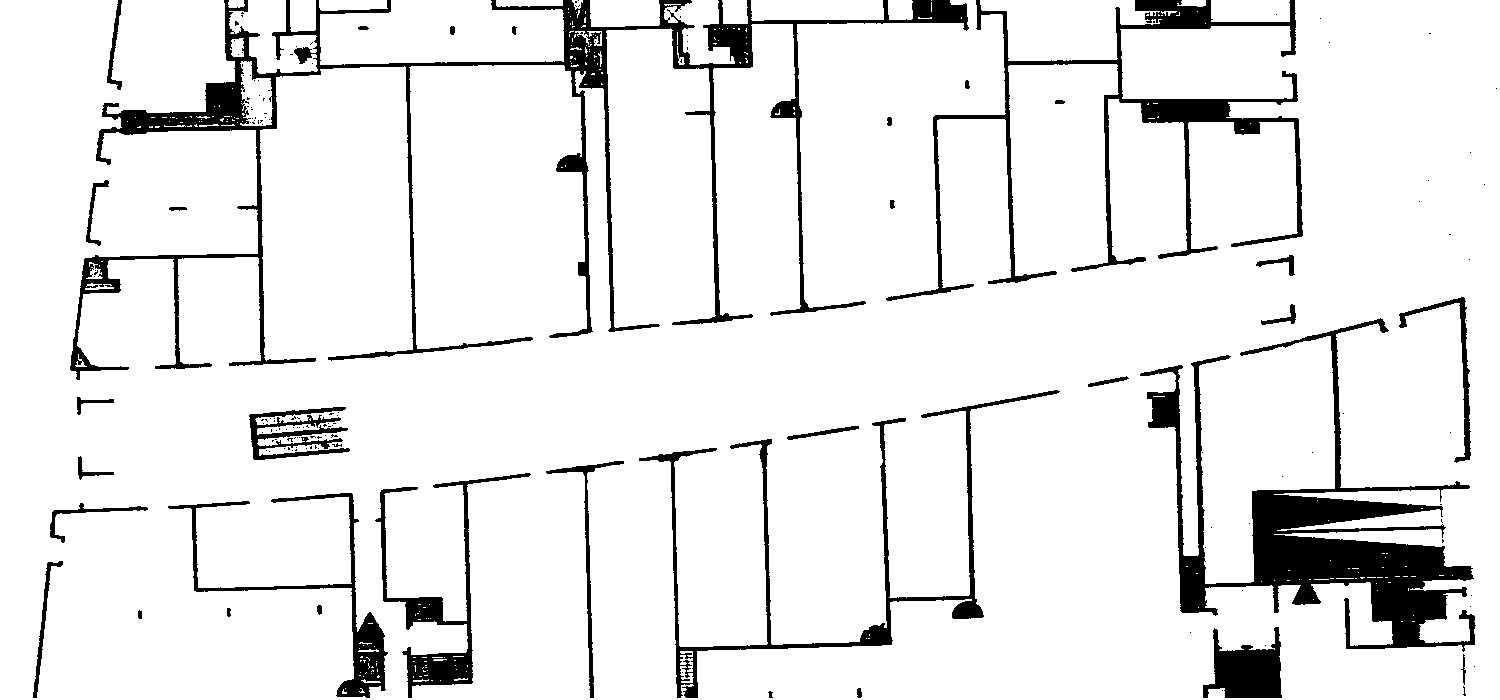
\includegraphics[width=0.95\textwidth]{Rive1.png}
\caption{2D map of the \emph{Rive de l'orne} shopping center.}
\label{fig:stage}
\end{figure}


In the Stage simulator the following map of the \emph{Rive de l'orne} shopping center has been realized. In Figure \ref{fig:stage} a section of the shopping mall in which we will deploy the prototypes is shown.
Additional maps have been realized for reproducing the environments of the partners in which some experiments will be performed.

The Stage environment models one or more robots that have the same 2D sensor and actuator configurations of the real ones and some additional mobile obstacles that represent people moving in the environment. Several behaviors can be tested in this simulated environment such as: 2D perception of human behaviors, human-robot social navigation (e.g., following a person or guiding a person), safe navigation in the environment.

The Stage environment has been fully realized and tested and this configuration will be used as a reference also for the development of the real robotic system.

\section{Data sets}

A number of data sets have been acquired in order to test sensor processing modules. In particular, data are collected from laser range finder and RGBD cameras mounted on the robot and represents people moving around and approaching the robot.

\begin{figure}
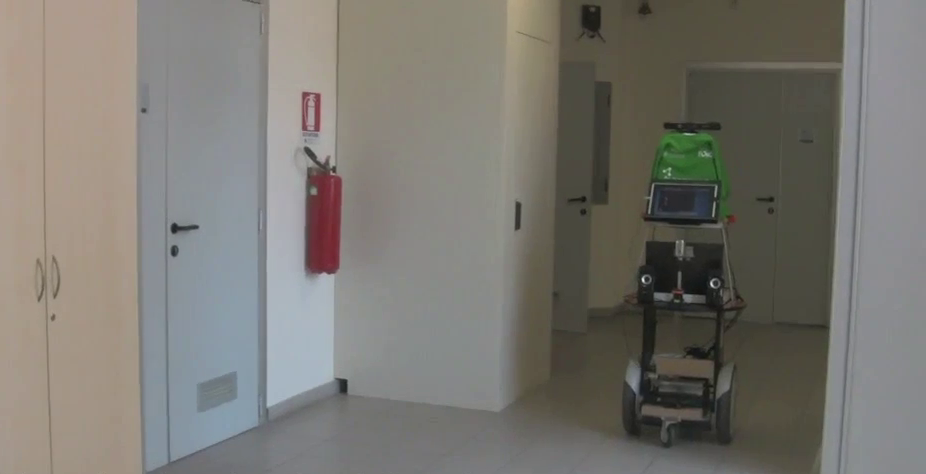
\includegraphics[width=0.95\textwidth]{diago.png}
\caption{Diago robot at Sapienza University of Rome.}
\label{fig:diago}
\end{figure}


The data sets have been captured with the mobile robot Diago in the Dept. of Computer, Control and Management Engineering, at Sapienza University of Rome (see Figure \ref{fig:diago}). Moreover, University of Caen will collect data in the same format with a similar robot in the \emph{Rive de l'orne} shopping mall.

The data sets will be made available soon to the all the partners in order to develop and test sensor processing components.

\section{Version management system}

In order to manage the development of the software by all the partners of the project, we have supported the team from University of Caen in the set up of a GIT repository for the software.
The repository is accessible only by the project partners and it is organized as follows.

The 'coaches/software' folder contains source code, libraries and binary code 
divided in the following sub-folders:

\begin{itemize}
\item \emph{src}:       contains (non-ROS) source code maintained in the coaches repository
\item \emph{ros}:       contains ros modules
\item \emph{external}:  contains external software not maintained in the coaches repository
\item \emph{bin}:       contains executable files
\item \emph{include}:   contains include files 
\item \emph{lib}:       contains libraries
\end{itemize}


The \emph{ros} folder contains a Catkin workspace (which is the standard building environment in ROS) and the following ROS packages, including the robotic software components described above.

\begin{itemize}
\item \emph{hello\_coaches\_developers}: a test package to check correct installation and set-up of the environment;
\item \emph{t11\_kb\_modeling}: software developed for Task T1.1;
\item \emph{t12\_kb\_reasoning}: software developed for Task T1.2;
\item \emph{t21\_image\_processing}: software developed for Task T2.1;
\item \emph{t22\_situation\_awareness}: software developed for Task T2.2;
\item \emph{t31\_multimodal\_hri}: software developed for Task T3.1;
\item \emph{t32\_human\_needs\_estimation}: software developed for Task T3.2;
\item \emph{t41\_robust\_navigation}: software developed for Task T4.1;
\item \emph{t42\_multi\_robot\_planning}: software developed for Task T4.2;
\end{itemize}


Moreover, additional packages developed outside the COACHES project are present in the \emph{external} directory and linked in the ROS Catkin workspace.
Some examples of these external packages are:
\begin{itemize}
\item \emph{gradient\_based\_navigation}: a package for safe navigation and obstacle avoidance in dynamic environments;
\item \emph{PetriNetPlans}: library and ROS bridge for plan execution;
\item \emph{stage\_environments}: a package for 2D simulation.
\end{itemize}

Automated scripts for initializing, setting-up, updating, building and testing the software environment have been developed and described in the repository. These scripts facilitate updates and testing and thus in  general the integration of functionalities developed by the different developers.

\begin{itemize}
\item \emph{coaches\_init}: initialize the software development environment (to be run once in every computer used for development);
\item \emph{coaches\_setup}:   set up all the system variables needed for development (to be run on every shell used for development);
\item \emph{coaches\_update}:  update of all the software from the GIT repository to the local workspace;
\item \emph{coaches\_make}:   build all the software
\end{itemize}

\section{Test}

The software environment has been succesfully tested by different developers from different partners using different machines, including laptops running the software for the real robots.

\end{document}
